\documentclass{beamer}
\usepackage[utf8]{inputenc}

\usetheme{Madrid}
\usecolortheme{default}
\usepackage{amsmath,amssymb,amsfonts,amsthm}
\usepackage{txfonts}
\usepackage{tkz-euclide}
\usepackage{listings}
\usepackage{adjustbox}
\usepackage{array}
\usepackage{tabularx}
\usepackage{gvv}
\usepackage{lmodern}
\usepackage{circuitikz}
\usepackage{tikz}
\usepackage{graphicx}

\setbeamertemplate{page number in head/foot}[totalframenumber]

\usepackage{tcolorbox}
\tcbuselibrary{minted,breakable,xparse,skins}

\definecolor{bg}{gray}{0.95}
\DeclareTCBListing{mintedbox}{O{}m!O{}}{%
  breakable=true,
  listing engine=minted,
  listing only,
  minted language=#2,
  minted style=default,
  minted options={%
    linenos,
    gobble=0,
    breaklines=true,
    breakafter=,,
    fontsize=\small,
    numbersep=8pt,
    #1},
  boxsep=0pt,
  left skip=0pt,
  right skip=0pt,
  left=25pt,
  right=0pt,
  top=3pt,
  bottom=3pt,
  arc=5pt,
  leftrule=0pt,
  rightrule=0pt,
  bottomrule=2pt,
  toprule=2pt,
  colback=bg,
  colframe=orange!70,
  enhanced,
  overlay={%
    \begin{tcbclipinterior}
    \fill[orange!20!white] (frame.south west) rectangle ([xshift=20pt]frame.north west);
    \end{tcbclipinterior}},
  #3,
}
\lstset{
    language=C,
    basicstyle=\ttfamily\small,
    keywordstyle=\color{blue},
    stringstyle=\color{orange},
    commentstyle=\color{green!60!black},
    numbers=left,
    numberstyle=\tiny\color{gray},
    breaklines=true,
    showstringspaces=false,
}
%------------------------------------------------------------
%This block of code defines the information to appear in the
%Title page
\title %optional
{2.2.18}
%\subtitle{A short story}

\author % (optional)
{R Nikhil-AI25BTECH11025}

\begin{document}

\frame{\titlepage}
\begin{frame}{Question}
\section*{2.2.18}
The unit vector normal to the plane 

$ x + 2y + 3z - 6 = 0 $

is:
\end{frame}

\begin{frame}{Theoretical Solution}
The normal vector to the plane is 
\begin{align}
\vec{n} = \myvec {1 \\ 2 \\ 3} 
\end{align}

The magnitude of $\vec{n}$ is
\begin{align}
\|\vec{n}\| = \sqrt{1^2 + 2^2 + 3^2} = \sqrt{14}.
\end{align}
\end{frame}

\begin{frame}{Theoretical Solution}
Therefore, the unit normal vectors are
\begin{align}
\pm \frac{\vec{n}}{\|\vec{n}\|}
= \pm \frac{1}{\sqrt{14}}
\myvec {1 \\ 2 \\ 3}
\end{align}

\end{frame}

\begin{frame}[fragile]
\frametitle{Main C Code}
   \begin{lstlisting}
#include <stdio.h>
#include <math.h>

double magnitude(int x, int y, int z) {
    return sqrt(x*x + y*y + z*z);
}

void unitVector(int x, int y, int z) {
    double mag = magnitude(x, y, z);
    printf("Unit normal vector = (%.3f)i + (%.3f)j + (%.3f)k\n", 
           x/mag, y/mag, z/mag);
}

int main() {
    int a = 1, b = 2, c = 3;  // coefficients of x, y, z
    unitVector(a, b, c);
    return 0;
}

   \end{lstlisting}
	\end{frame}

\begin{frame}[fragile]
\frametitle{C Function}
   \begin{lstlisting}
#include <math.h>

double magnitude(int x, int y, int z) {
    return sqrt(x*x + y*y + z*z);
}

void unitVector(int x, int y, int z, double *ux, double *uy, double *uz) {
    double mag = magnitude(x, y, z);
    *ux = x / mag;
    *uy = y / mag;
    *uz = z / mag;
}

\end{lstlisting}
\end{frame}

\begin{frame}[fragile]
\frametitle{Python Code}
   \begin{lstlisting}
import ctypes
import numpy as np
import matplotlib.pyplot as plt
from mpl_toolkits.mplot3d import Axes3D

# === Load the C shared library ===
lib = ctypes.CDLL("./libunitvector.so")

# Define C function signature
lib.unitVector.argtypes = (ctypes.c_int, ctypes.c_int, ctypes.c_int,
                           ctypes.POINTER(ctypes.c_double),
                           ctypes.POINTER(ctypes.c_double),
                           ctypes.POINTER(ctypes.c_double))
lib.unitVector.restype = None

   \end{lstlisting}
\end{frame}

\begin{frame}[fragile]
\frametitle{Python Code}
   \begin{lstlisting}
# Plane equation: ax + by + cz + d = 0
a, b, c, d = 1, 2, 3, -6   # Example: x + 2y + 3z - 6 = 0

# Output variables for unit vector
ux = ctypes.c_double()
uy = ctypes.c_double()
uz = ctypes.c_double()

# Call C function to get unit normal vector
lib.unitVector(a, b, c, ctypes.byref(ux), ctypes.byref(uy), ctypes.byref(uz))
u = np.array([ux.value, uy.value, uz.value])

# === Plotting ===
fig = plt.figure()
ax = fig.add_subplot(111, projection='3d')

\end{lstlisting}
\end{frame}

\begin{frame}[fragile]
\frametitle{Python Code}
   \begin{lstlisting}
# Create mesh grid for the plane
xx, yy = np.meshgrid(range(-2, 5), range(-2, 5))
zz = (-(a*xx + b*yy + d)) / c   # Solve for z from ax+by+cz+d=0

# Plot the plane
ax.plot_surface(xx, yy, zz, alpha=0.5, color='cyan')

# Pick a point on the plane (x=0,y=0  z=-d/c)
point = np.array([0, 0, -d/c])

# Plot the normal vector
ax.quiver(point[0], point[1], point[2],
          u[0], u[1], u[2],
          length=2, color='red', linewidth=2)
 \end{lstlisting}
\end{frame}  

\begin{frame}[fragile]
\frametitle{Python Code}
   \begin{lstlisting}
ax.set_xlabel("X")
ax.set_ylabel("Y")
ax.set_zlabel("Z")
ax.set_title("Plane and its Unit Normal Vector")
plt.savefig("/home/r-nikhil/ee1030-2025/ai25btech11025/matgeo/2.2.18/figsplotc.png")
plt.show()
\end{lstlisting}
\end{frame}

\begin{frame}{Plot}
\begin{figure}[h!]
    \centering
    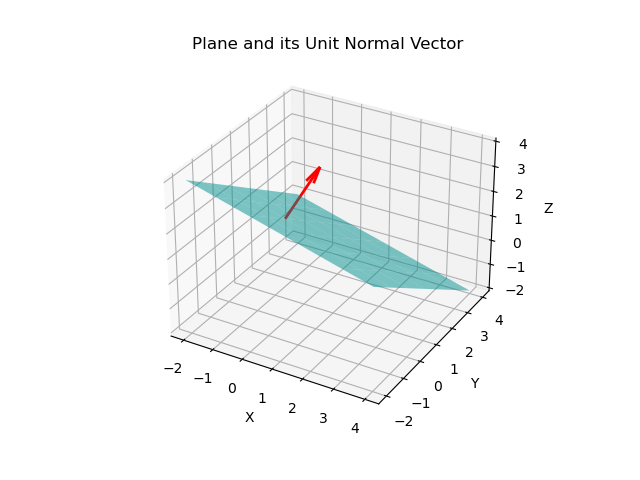
\includegraphics[height=0.6\textheight, keepaspectratio]{figs/plotc.png}
    \label{figure_1}
\end{figure}

\end{frame}

\end{document}
